\documentclass[11pt]{article}
\usepackage[margin=1in]{geometry}
\usepackage{graphicx}
\usepackage{booktabs}
\usepackage{amsmath,amssymb}
\usepackage[hidelinks]{hyperref}
\usepackage{microtype}
\usepackage{caption}

\title{\textbf{Cytochrome P450 Inhibitor Classification Revisited:\\
A Decade of Algorithmic, Representational, and AI-Coordinated Uplift}}
\author{Daniel E. Siegle\\
\small Extension to \emph{Cytochrome P450 Inhibitor Classification with Statistical Learning} (M.S.\ Thesis, NCCU, 2015)}
\date{November 2026}

\begin{document}
\maketitle

\begin{abstract}
In my 2015 master's thesis, I compared a proprietary Bayesian Binary QSAR classifier from the Molecular Operating Environment (MOE) against three freely available Python classifiers ($k$-nearest neighbors, random forests, and support vector machines) on PubChem Bioassay AID1851 across five cytochrome P450 (CYP) isozymes (1A2, 2C9, 2C19, 2D6, and 3A4). That work showed that open-source learners could outperform an industry-standard proprietary classifier on the same 186 MOE 2D descriptors (mean held-out Test ROC-AUC 0.8416 for the best 2015 baseline, SVM), while leaving three open questions: whether observed gains were statistically significant, what neural and ensemble architectures would achieve, and whether proprietary descriptors themselves remained necessary.

Eleven years later, I revisit the exact 2015 Figshare training and held-out test splits---evaluating every model on 100\% of every test set under a strict, zero-leakage 5-fold cross-validation protocol---to quantify the uplift delivered by a decade of progress in libraries, methods, cloud GPU compute, and AI-assisted research coordination. Across four structured tiers spanning 30 model variants (gradient-boosted trees, Tanimoto and hybrid kernel SVMs, 5-head multi-task residual neural networks, bond-aware graph neural networks, end-to-end fine-tuned molecular transformers, and nested meta-stacking), mean Test ROC-AUC rises from \textbf{0.8416} to \textbf{0.8792} (\textbf{+0.0375}, exact DeLong $p \le 2.7 \times 10^{-7}$ on all five isozymes; $p = 2.0 \times 10^{-25}$ on 3A4), mean Test Accuracy rises from \textbf{76.40\%} to \textbf{80.63\%} (exact McNemar $p \le 3.5 \times 10^{-5}$ on all five), and mean Brier score drops from \textbf{0.1601} to \textbf{0.1388} (mean 10-bin ECE 0.0216). Decomposing this gain shows that \textbf{52\%} (+0.0196) comes from modern tabular algorithms and stacking on the unchanged 2015 MOE descriptors, \textbf{37\%} (+0.0138) from open-source RDKit fingerprints and kernels, and \textbf{11\%} (+0.0042, $p < 0.03$ on all five isozymes) from GPU-accelerated multi-task deep learning, GNNs, and pretrained SMILES transformers. Crucially, a \textbf{100\% open-source stack} using zero MOE descriptors reaches \textbf{0.8777} mean AUC, rendering proprietary MOE descriptors statistically redundant ($p \in [0.059, 0.668]$ across all five isozymes). The entire multi-tier campaign was executed across a local CPU and cloud Tesla T4 GPU (1.80 Colab compute units) in roughly 3.5 hours of AI-coordinated wall-clock time, compared with an estimated 2--3 semesters for the original 2015 thesis.
\end{abstract}

\section{Introduction and Rationale}
When I completed my 2015 thesis on \emph{in silico} cytochrome P450 (CYP) inhibition modeling, freely available \texttt{scikit-learn} classifiers outperformed MOE's proprietary Binary QSAR model on every isozyme, yet still depended on 186 proprietary MOE descriptors, modeled each isozyme in isolation despite known cross-isoform promiscuity (Veith et al., 2009), and omitted formal statistical significance testing and scaffold-split validation. Revisiting the exact 2015 Figshare splits eleven years later provides a clean controlled experiment: holding the compounds, activity threshold ($\text{ActivityScore} \ge 40$), and test sets strictly fixed allows us to decompose ten years of uplift into (i)~updated libraries and defaults, (ii)~modern tabular algorithms and open-source cheminformatics representations, (iii)~accessible cloud GPU compute for multi-task representation learning, and (iv)~AI-assisted research coordination.

\section{Data and Zero-Leakage Validation Protocol}
All models use the exact 2015 training and test splits for CYP 1A2 ($9{,}600 / 2{,}400$), 2C9 ($6{,}593 / 1{,}649$), 2C19 ($9{,}462 / 2{,}366$), 2D6 ($4{,}433 / 1{,}109$), and 3A4 ($8{,}427 / 2{,}107$). Unique PubChem SIDs ($16{,}725$) were mapped to canonical SMILES and Bemis--Murcko scaffolds; the 22 SIDs ($\approx 0.13\%$) lacking SMILES are retained in every evaluation via fold-median descriptor imputation, zero fingerprint vectors, dummy single-node graphs, and empty SMILES token sequences so that \textbf{100\% of every test set} is scored.

Internal validation uses identical 5-fold \texttt{StratifiedKFold(n\_splits=5, shuffle=True, random\_state=0)} splits across all tiers. All imputers, scalers (\texttt{StandardScaler}, \texttt{QuantileTransformer}), and rare-bit filters ($\text{count} \ge 5$) are fit strictly inside each training fold. For 5-head multi-task models (Tiers 2B, 3A, 3B), all SIDs in \texttt{test\{iso\}.csv} are excluded from the entire 5-head master pool, and within each fold $k$ all fold-$k$ validation SIDs are excluded from all five heads (verified by runtime assertions; Figure~\ref{fig:arch}B).

\begin{figure}[htbp]
  \centering
  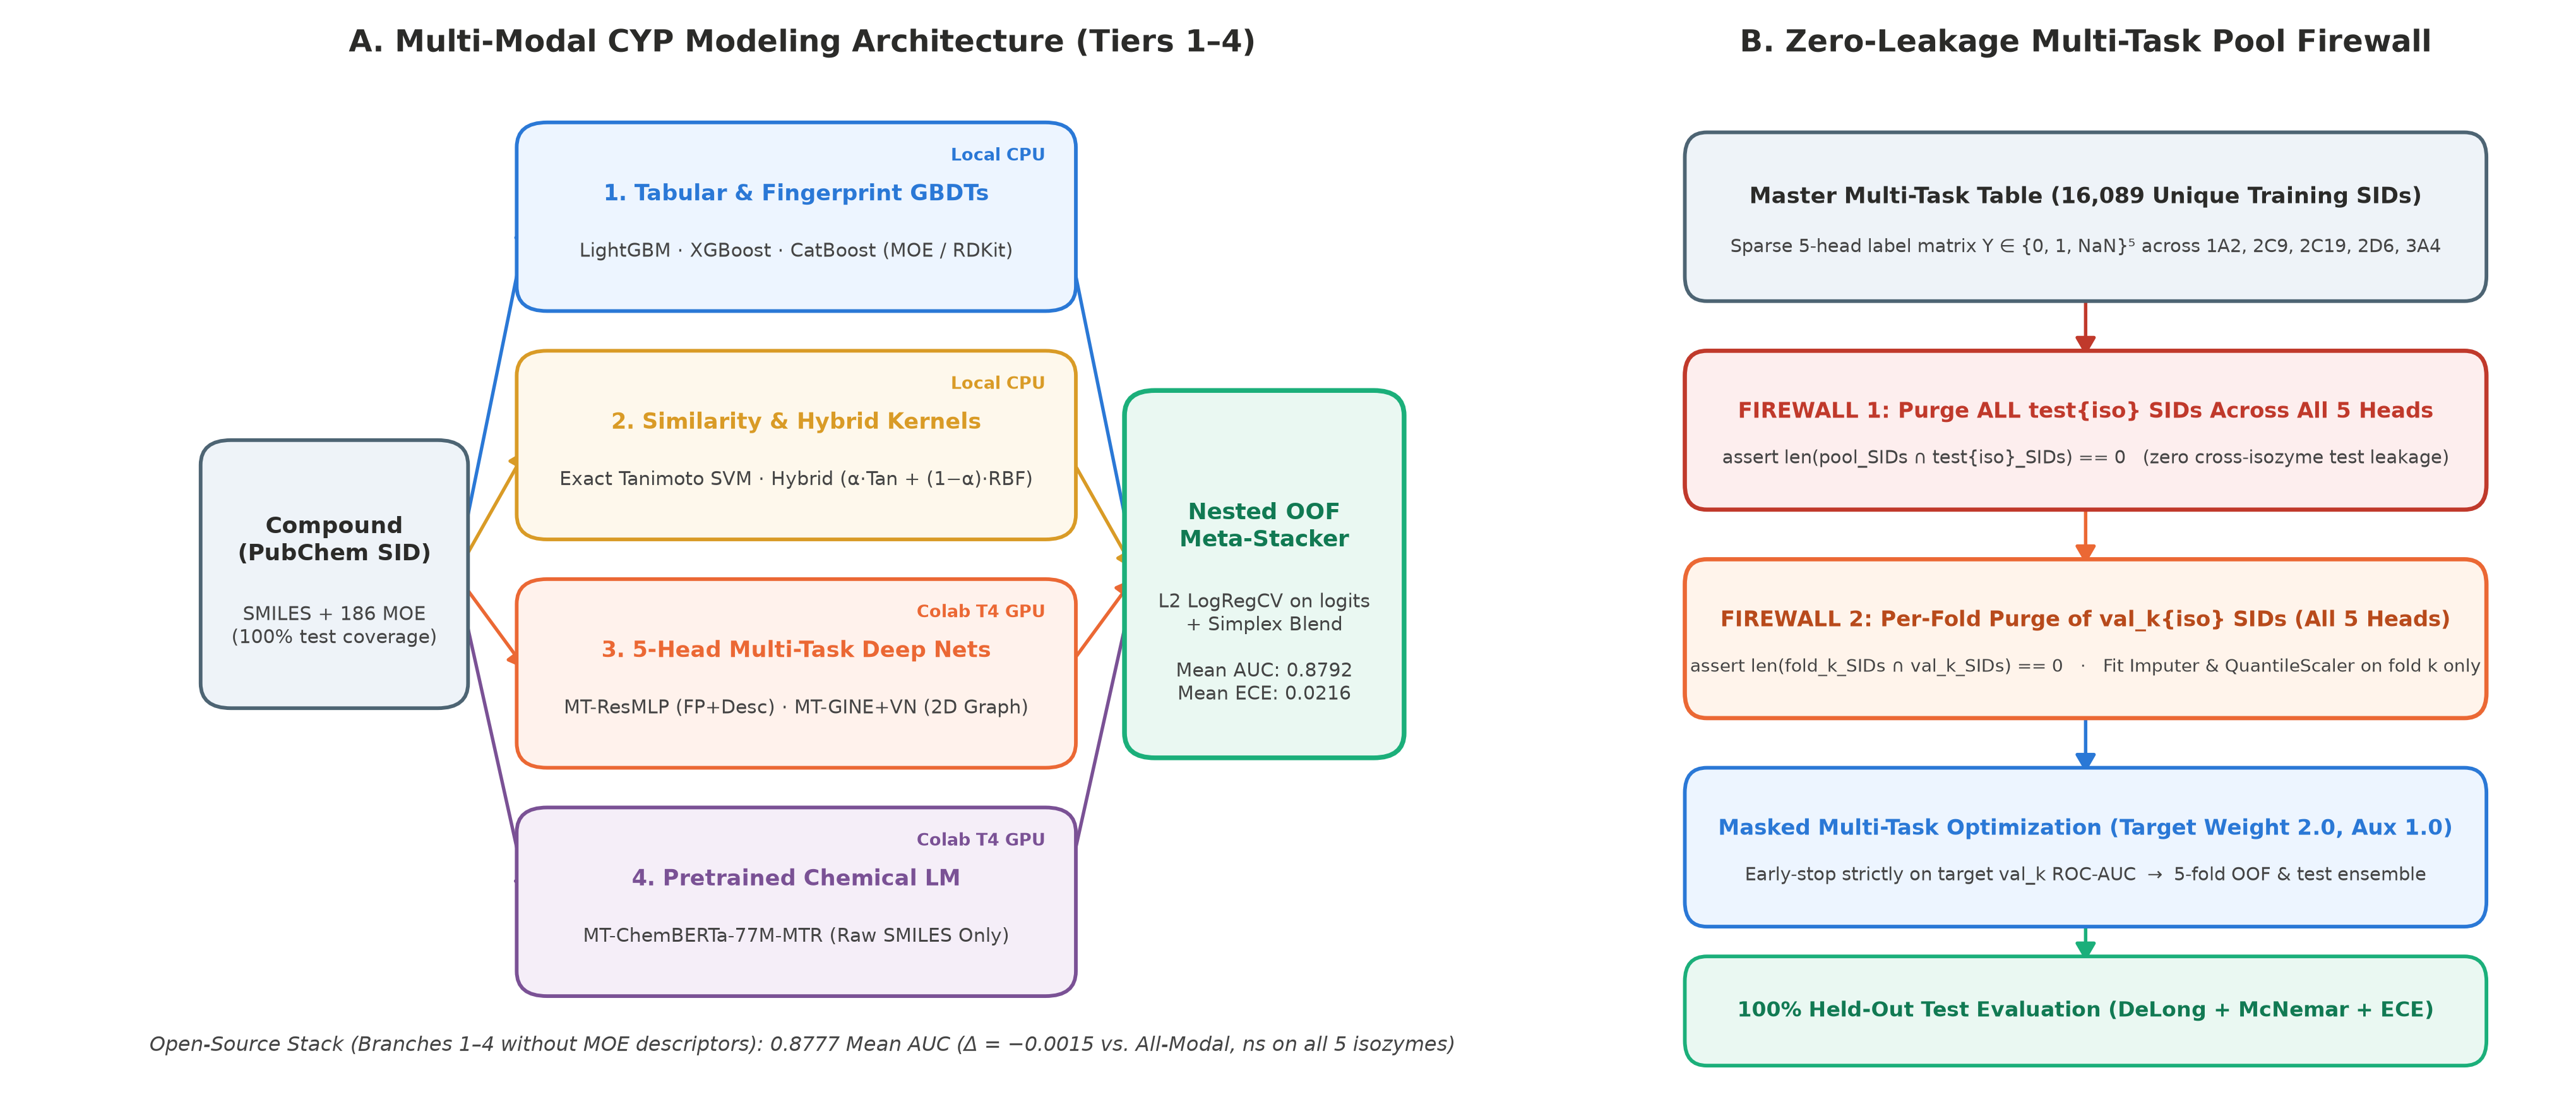
\includegraphics[width=\textwidth]{img/fig7_architecture_and_leakage.png}
  \caption{(A) Four-branch multi-modal architecture feeding the nested out-of-fold meta-stacker across local CPU and Colab Tesla T4 GPU. (B) Double-firewall multi-task isolation protocol guaranteeing zero cross-isozyme test or validation leakage.}
  \label{fig:arch}
\end{figure}

\section{Mathematical Formulation of Key Methods}
For binary RDKit fingerprint matrices $A \in \{0,1\}^{n \times d}$ and $B \in \{0,1\}^{m \times d}$ ($d = 5{,}287$), the exact Tanimoto kernel and its hybrid combination with a fold-scaled continuous descriptor RBF kernel ($\tilde{\mathbf{u}}_{\text{desc}} \in \mathbb{R}^{403}$) are:
\begin{equation}
  K_{\text{Tan}}(A,B)_{ij} = \frac{\mathbf{a}_i^\top \mathbf{b}_j}{\|\mathbf{a}_i\|_1 + \|\mathbf{b}_j\|_1 - \mathbf{a}_i^\top \mathbf{b}_j}, \qquad
  K_{\text{hyb}}(\mathbf{u},\mathbf{v}) = \alpha K_{\text{Tan}} + (1-\alpha)\exp\!\left(-\gamma\|\tilde{\mathbf{u}}_{\text{desc}} - \tilde{\mathbf{v}}_{\text{desc}}\|_2^2\right).
\end{equation}
Multi-task neural networks (Tiers 2B, 3A, 3B) optimize a masked, task-weighted binary cross-entropy loss over sparse 5-head labels $y_{it}$ with mask $m_{it} \in \{0,1\}$ ($w_{t^*}=2.0$ for the target isozyme, $w_t=1.0$ for auxiliary heads):
\begin{equation}
  \mathcal{L}_{\text{MT}} = \frac{\sum_{i \in \mathcal{B}} \sum_{t=1}^{5} m_{it}\, w_t\, \ell_{\text{BCE}}(\hat{z}_{it}, y_{it})}{\sum_{i \in \mathcal{B}} \sum_{t=1}^{5} m_{it}\, w_t}.
\end{equation}
In Tier 3A, each GINE layer updates atom representation $\mathbf{h}_v^{(\ell)}$ using a global virtual node $\mathbf{g}^{(\ell)}$ and incident bond embeddings $\mathbf{e}_{uv}$:
\begin{equation}
  \mathbf{h}_v^{(\ell+1)} = \operatorname{LayerNorm}\!\left(\mathbf{h}_v^{(\ell)} + \operatorname{MLP}^{(\ell)}\!\left((1+\epsilon^{(\ell)})\tilde{\mathbf{h}}_v^{(\ell)} + \sum_{u \in \mathcal{N}(v)} \operatorname{SiLU}(\tilde{\mathbf{h}}_u^{(\ell)} + \mathbf{e}_{uv})\right)\right), \quad \tilde{\mathbf{h}}_v^{(\ell)} = \mathbf{h}_v^{(\ell)} + \mathbf{g}^{(\ell)}.
\end{equation}
Finally, Tier 4 meta-stackers combine $M$ base probability predictions via nested-CV $L_2$ logistic regression on clipped log-odds, $\hat{p}_{\text{stack}}(x) = \sigma(\beta_0 + \sum_{m=1}^{M} \beta_m \operatorname{logit}(\hat{p}_m(x)))$, evaluated with Brier score, 10-bin ECE, exact Sun \& Xu (2014) DeLong ROC-AUC tests, and exact binomial McNemar tests.

\section{Results}
\subsection{Ten-Year Progression and Gain Decomposition}
Figure~\ref{fig:progression} and Table~\ref{tab:main} report held-out test performance across all five isozymes. Mean Test ROC-AUC climbs monotonically from 0.8126 (2015 10-tree RF) and 0.8416 (2015 SVM) to 0.8612 (Tier 1 MOE Stack), 0.8715 (Tier 2A RDKit-Only Stack), 0.8750 (Tier 2A MOE+RDKit Stack), 0.8777 (Tier 4 Grand Open-Source Stack), and \textbf{0.8792} (Tier 4 Grand All-Modal Stack/Blend; mean Test Accuracy \textbf{80.63\%}, mean Brier \textbf{0.1388}, mean 10-bin ECE \textbf{0.0216}).

\begin{figure}[htbp]
  \centering
  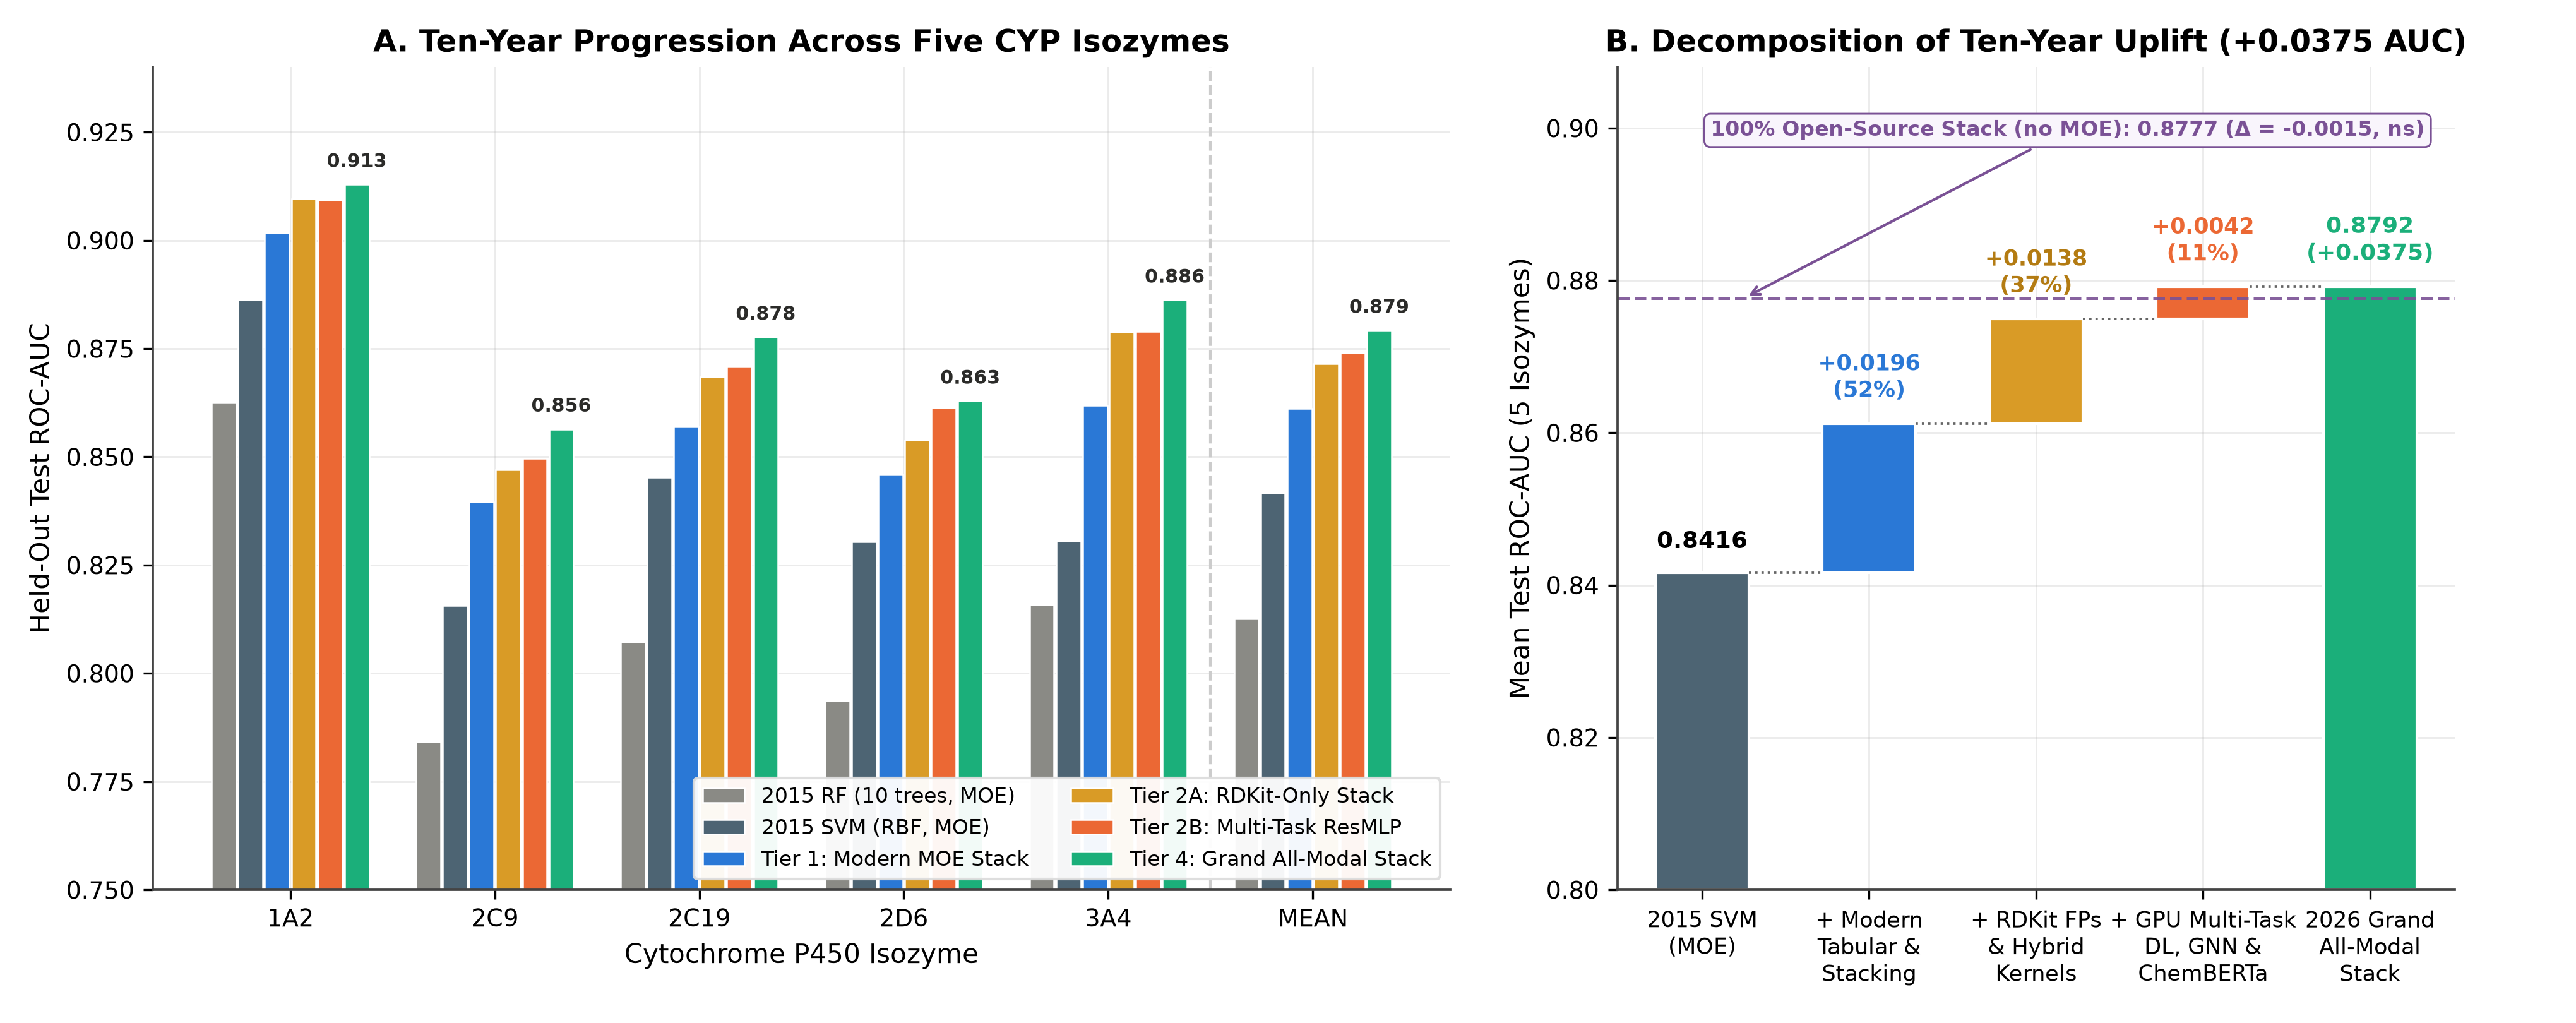
\includegraphics[width=\textwidth]{img/fig1_ten_year_progression.png}
  \caption{(A) Held-out Test ROC-AUC across all five CYP isozymes and their mean from 2015 baselines to 2026 multi-modal stacking. (B) Attribution waterfall decomposing the +0.0375 mean ROC-AUC gain over the 2015 SVM baseline.}
  \label{fig:progression}
\end{figure}

\begin{table}[htbp]
\centering
\scriptsize
\caption{Held-out test Accuracy / ROC-AUC across all five CYP isozymes (100\% test coverage).}
\label{tab:main}
\begin{tabular}{llccccccc}
\toprule
Tier & Model & 1A2 & 2C9 & 2C19 & 2D6 & 3A4 & Mean Acc & Mean AUC \\
\midrule
2015 MOE & \texttt{RF\_baseline} (10 trees) & 0.782 / 0.863 & 0.720 / 0.784 & 0.743 / 0.807 & 0.717 / 0.794 & 0.746 / 0.816 & 0.7413 & 0.8126 \\
2015 MOE & \texttt{SVM\_baseline} & 0.806 / 0.886 & 0.745 / 0.816 & 0.774 / 0.845 & 0.749 / 0.830 & 0.746 / 0.831 & 0.7640 & 0.8416 \\
Tier 1 MOE & \texttt{Stack\_LogReg} & 0.819 / 0.902 & 0.765 / 0.840 & 0.784 / 0.857 & 0.774 / 0.846 & 0.781 / 0.862 & 0.7848 & 0.8612 \\
Tier 2A RDKit & \texttt{Stack\_RDKit} & 0.834 / 0.910 & 0.772 / 0.847 & 0.802 / 0.868 & 0.788 / 0.854 & 0.795 / 0.879 & 0.7983 & 0.8715 \\
Tier 2A Comb. & \texttt{Stack\_MOE\_RDKit} & 0.831 / 0.911 & 0.773 / 0.852 & \textbf{0.808} / 0.874 & 0.785 / 0.857 & 0.798 / 0.881 & 0.7989 & 0.8750 \\
Tier 2B GPU & \texttt{MT\_ResMLP\_MOE\_RDKit} & 0.835 / 0.909 & 0.779 / 0.850 & 0.801 / 0.871 & 0.801 / 0.861 & 0.800 / 0.879 & 0.8030 & 0.8740 \\
Tier 3A GPU & \texttt{MT\_GNN\_GraphPlusDesc} & 0.813 / 0.895 & 0.758 / 0.836 & 0.777 / 0.852 & 0.761 / 0.839 & 0.764 / 0.846 & 0.7746 & 0.8535 \\
Tier 3B GPU & \texttt{MT\_ChemBERTa\_77M\_MTR} & 0.814 / 0.896 & 0.774 / 0.843 & 0.798 / 0.870 & 0.776 / 0.844 & 0.800 / 0.876 & 0.7923 & 0.8659 \\
Tier 4 Open & \texttt{Grand\_OpenSource\_Stack} & 0.834 / 0.912 & \textbf{0.784} / 0.856 & 0.805 / 0.876 & 0.803 / 0.861 & 0.799 / 0.885 & 0.8047 & 0.8777 \\
Tier 4 All & \texttt{Grand\_AllModal\_Stack} & \textbf{0.837} / \textbf{0.913} & 0.782 / 0.856 & 0.806 / 0.878 & 0.801 / 0.863 & \textbf{0.803} / \textbf{0.886} & 0.8056 & \textbf{0.8792} \\
Tier 4 All & \texttt{Grand\_AllModal\_Blend} & 0.835 / 0.912 & 0.783 / \textbf{0.857} & 0.807 / \textbf{0.878} & \textbf{0.808} / \textbf{0.863} & 0.799 / 0.886 & \textbf{0.8063} & \textbf{0.8792} \\
\bottomrule
\end{tabular}
\end{table}

\begin{figure}[htbp]
  \centering
  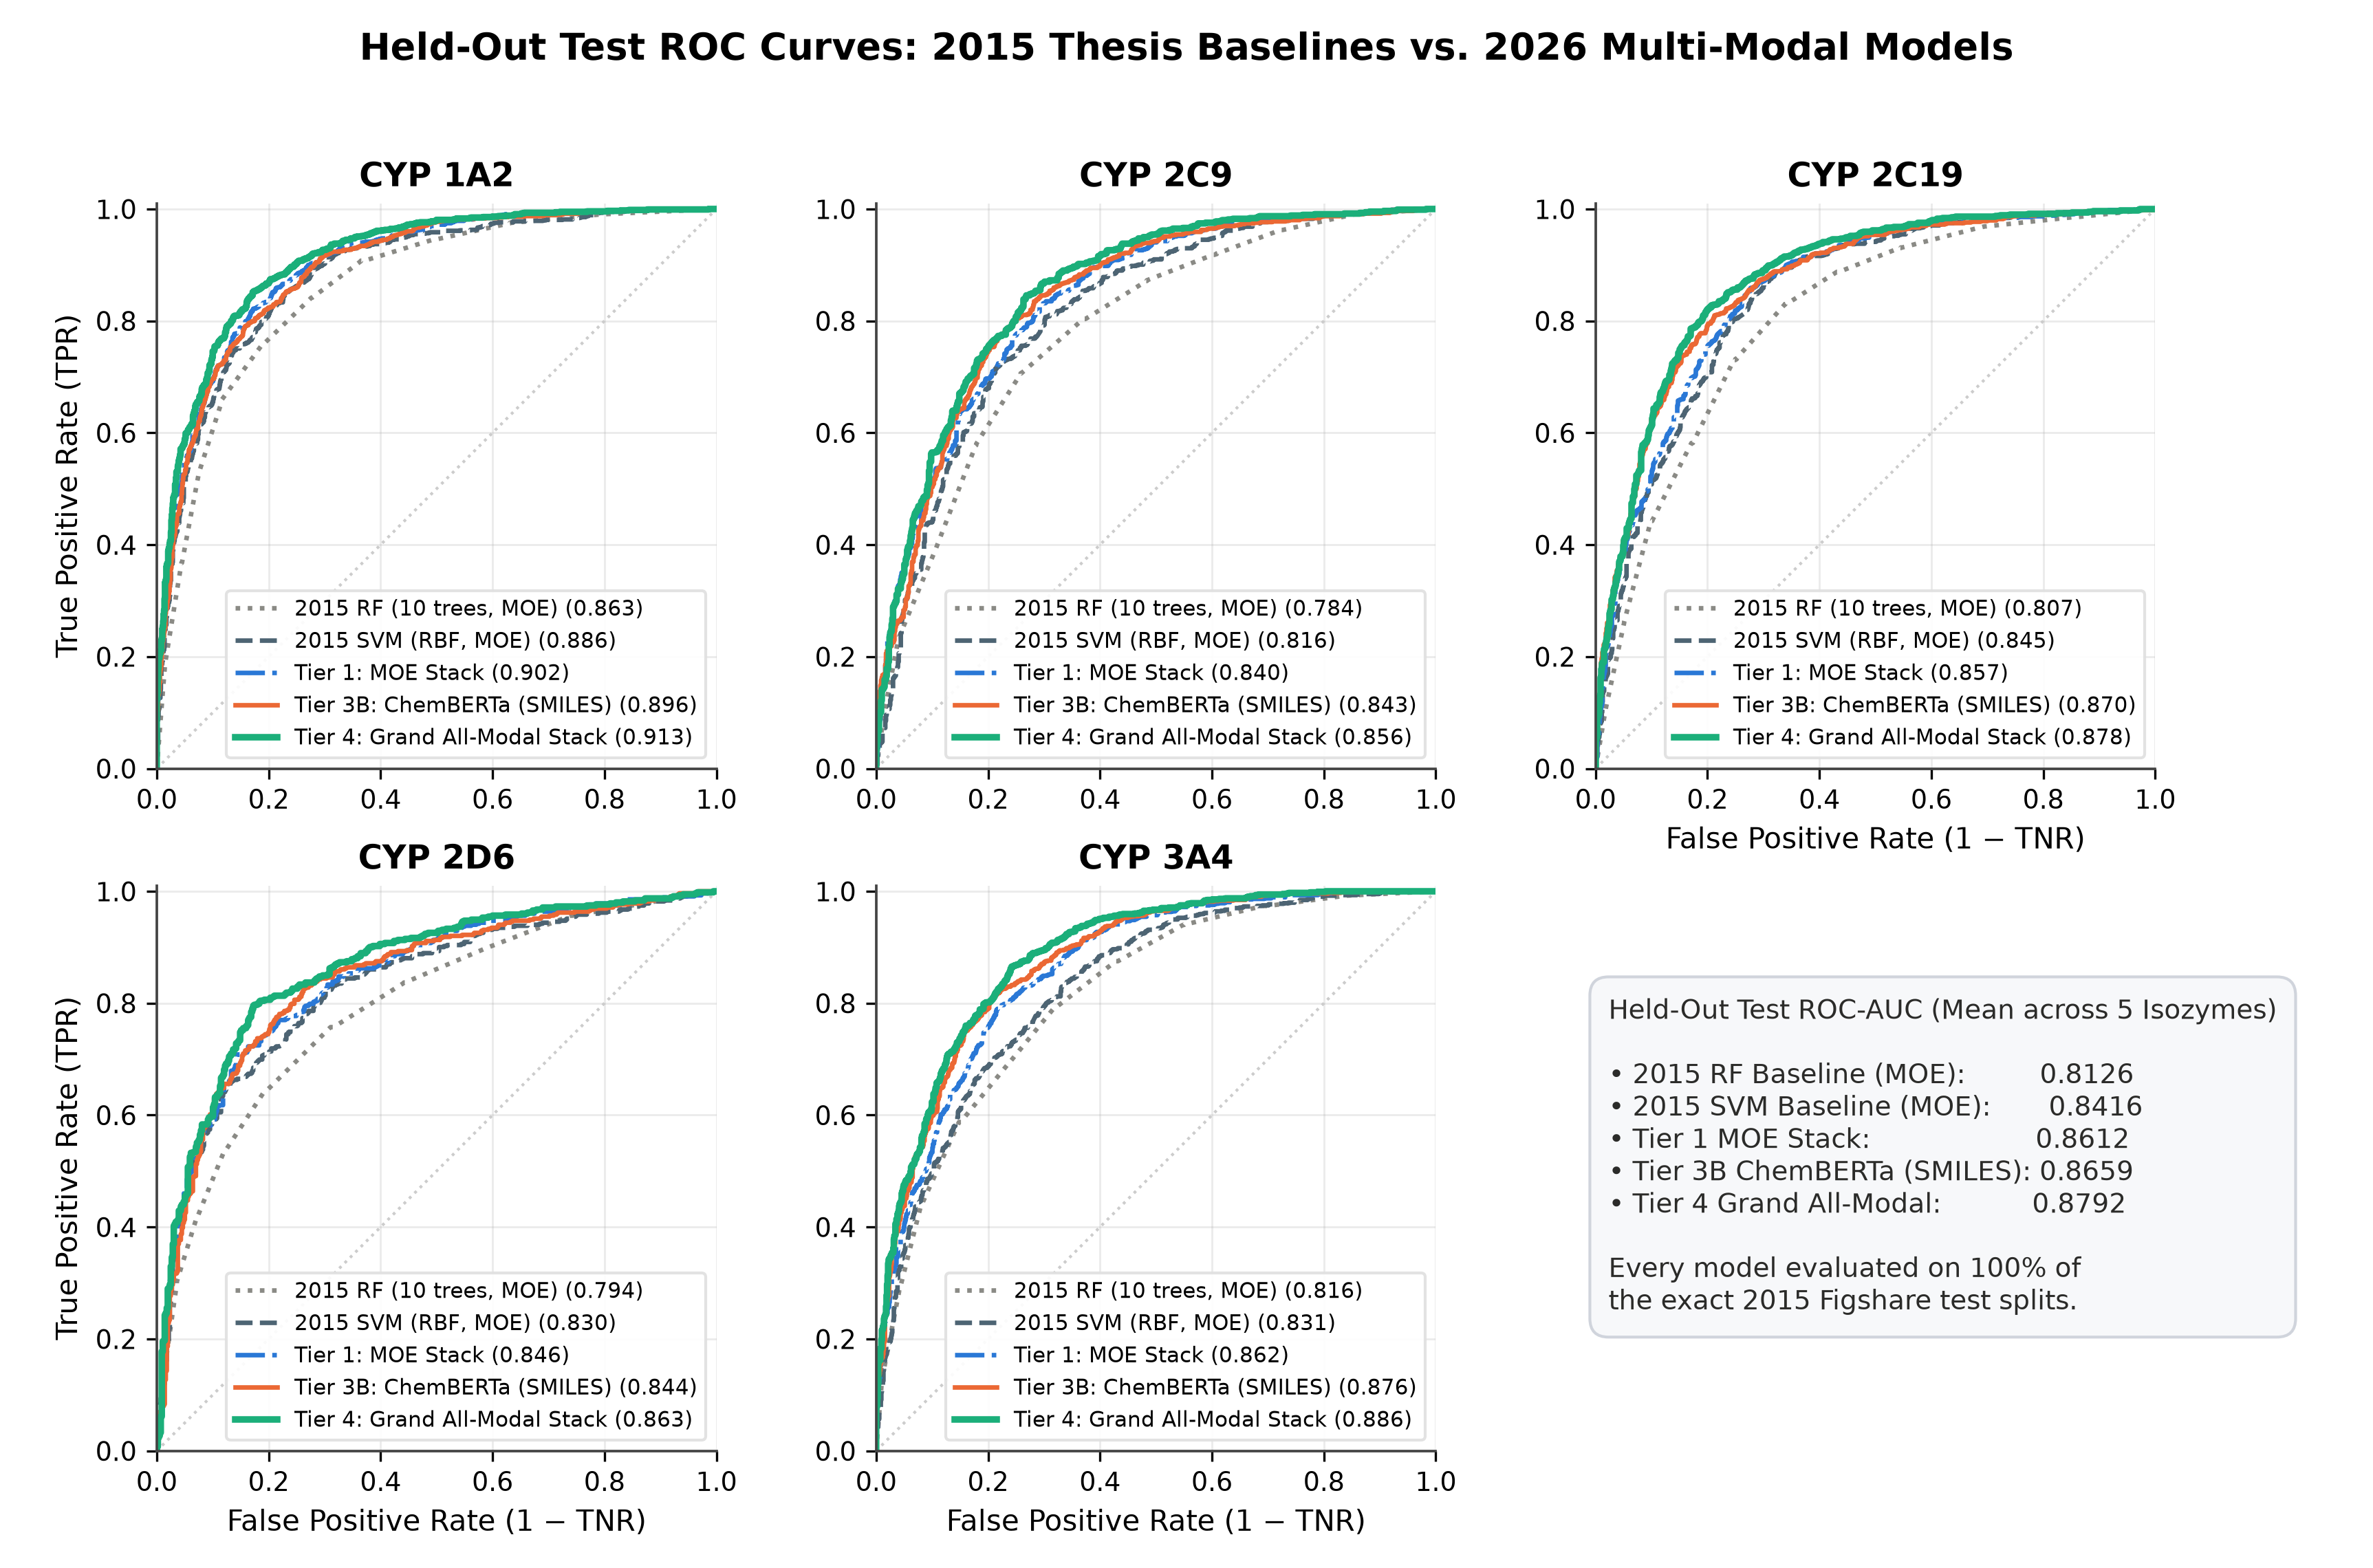
\includegraphics[width=0.95\textwidth]{img/fig2_roc_curves_decade.png}
  \caption{Held-out test ROC curves across all five CYP isozymes comparing 2015 baselines against 2026 Tier 1, Tier 3B (raw SMILES ChemBERTa), and Tier 4 Grand All-Modal models.}
  \label{fig:roc}
\end{figure}

\begin{figure}[htbp]
  \centering
  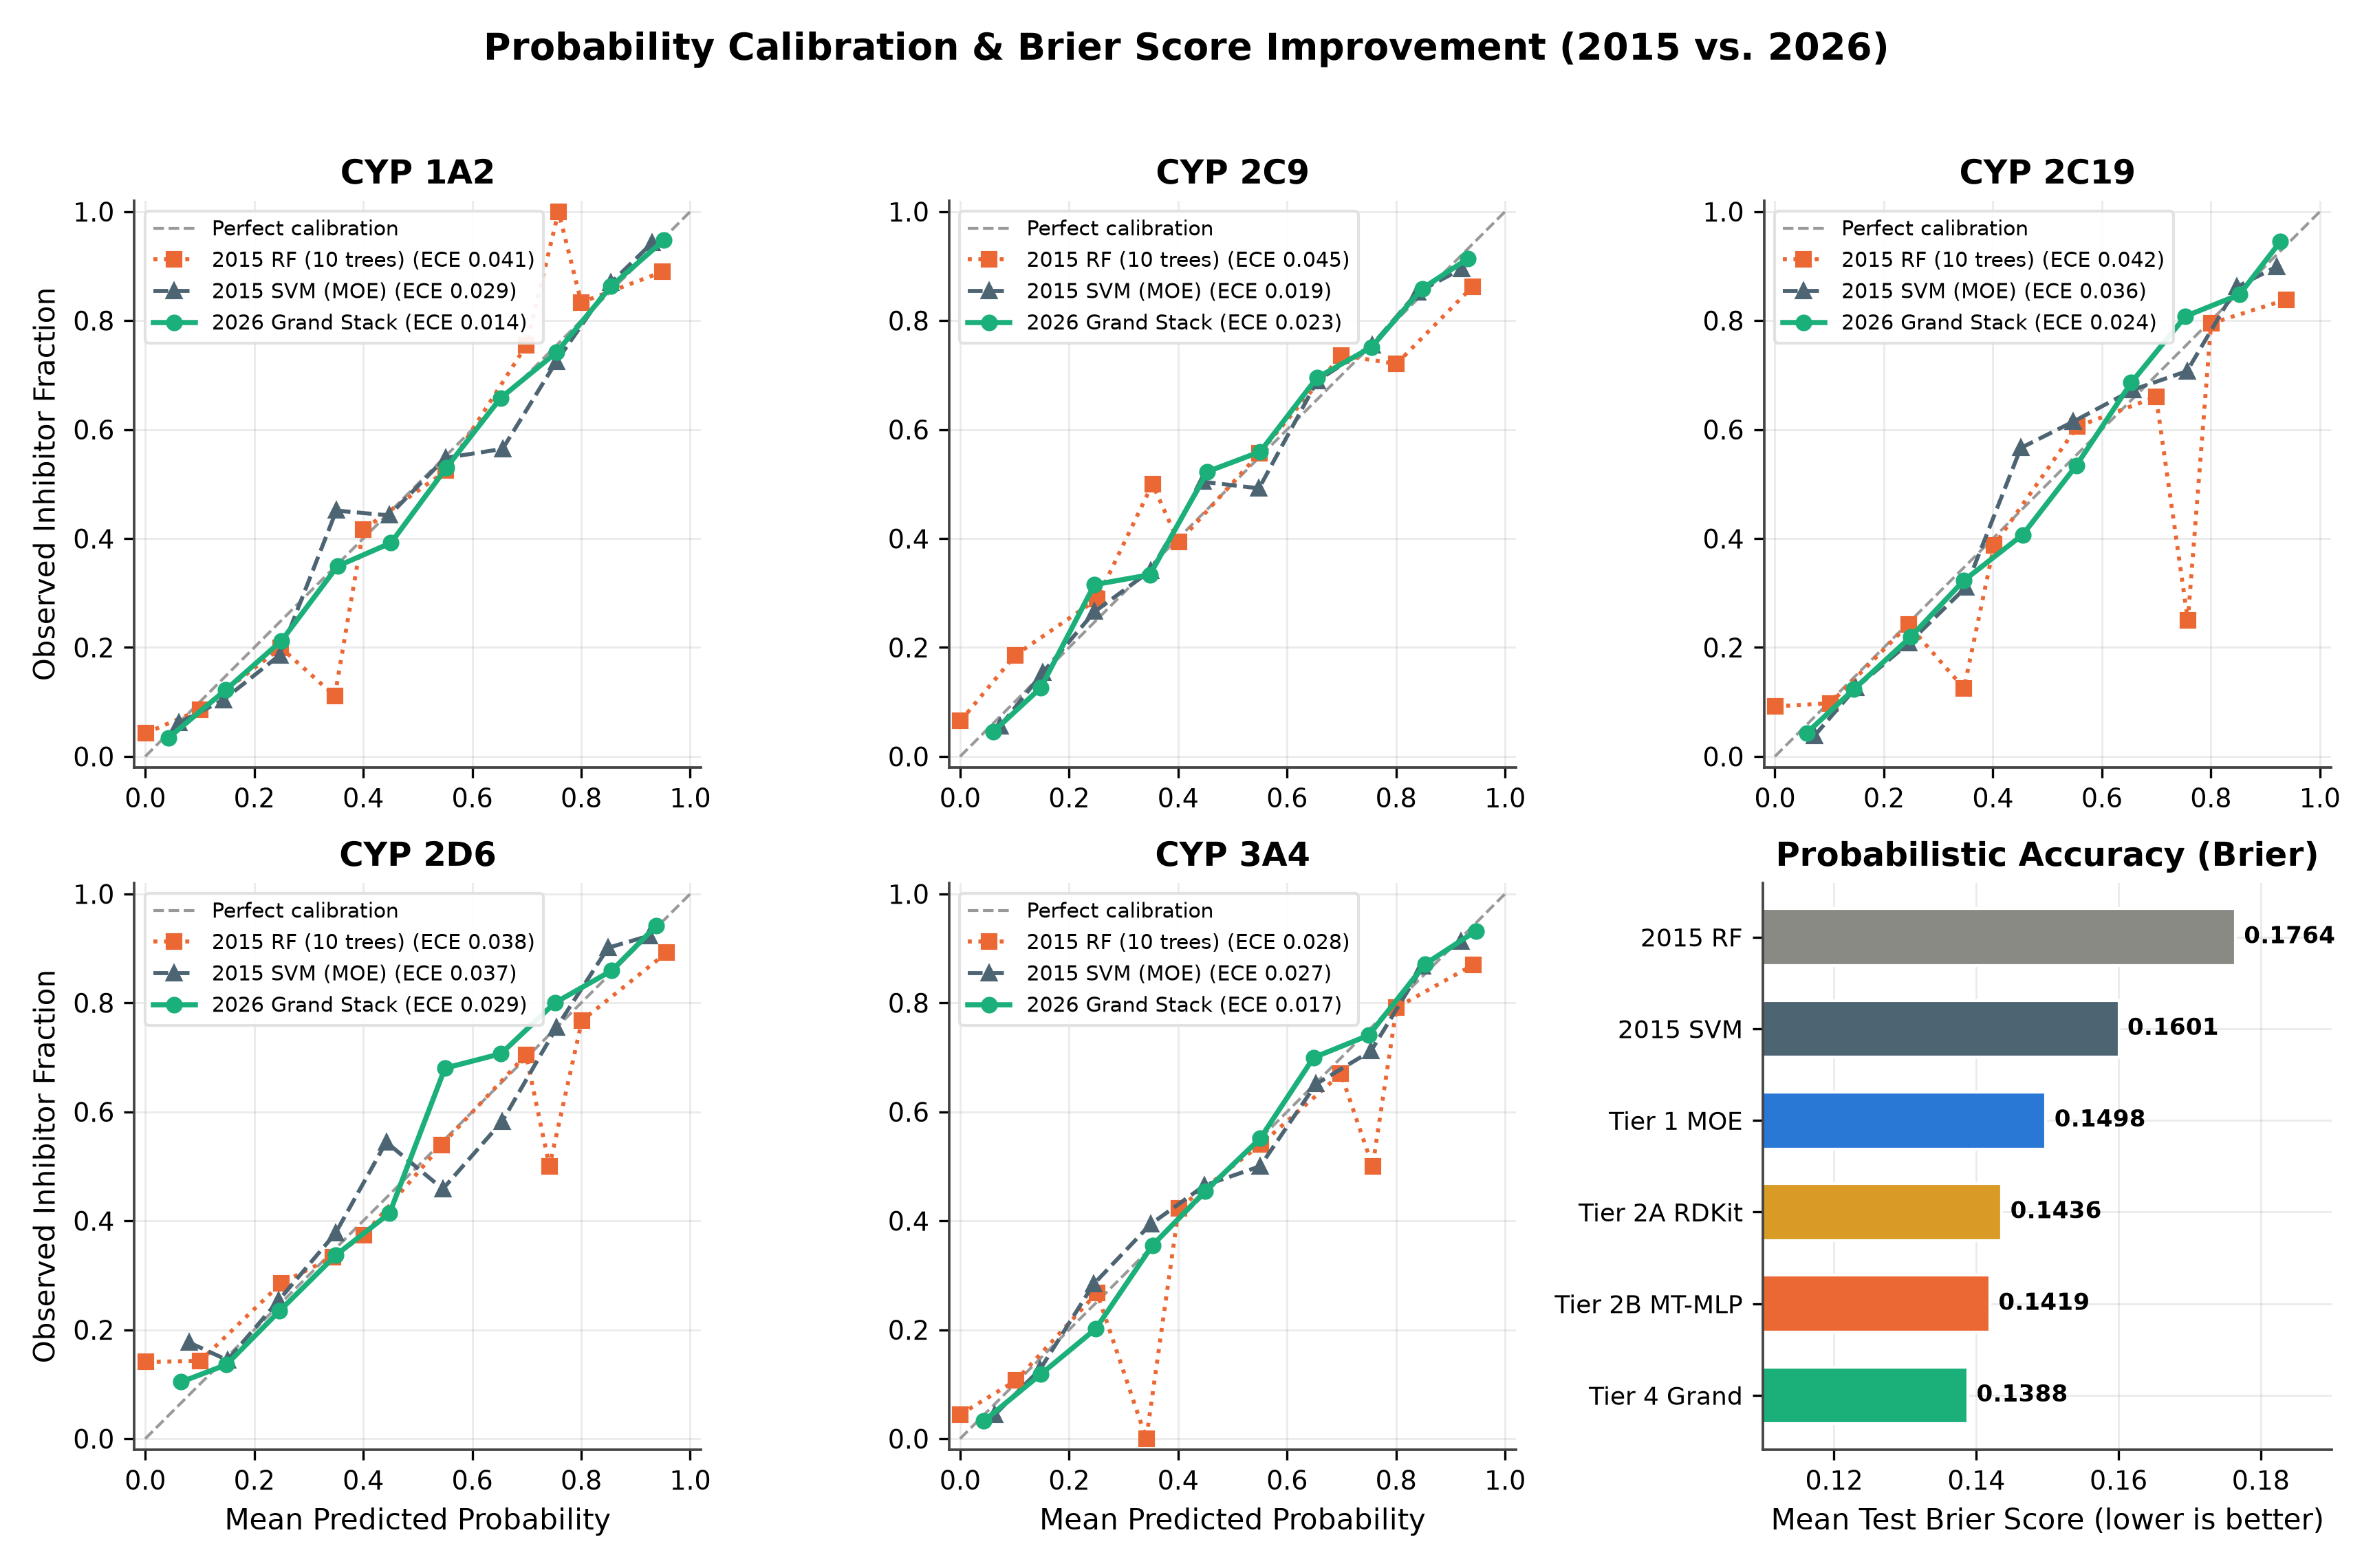
\includegraphics[width=0.95\textwidth]{img/fig3_calibration_reliability.png}
  \caption{Reliability diagrams and Brier score progression demonstrating substantially tighter probability calibration in 2026 (mean ECE 0.0216 vs.\ 0.0389 for 2015 RF).}
  \label{fig:cal}
\end{figure}

\subsection{Statistical Significance, Scaffold Generalization, and Modality Contributions}
Exact DeLong tests (Figure~\ref{fig:delong}) confirm that (A)~algorithm modernization on MOE descriptors is highly significant on all five isozymes ($p < 3 \times 10^{-4}$), (B)~the 100\% open-source Grand Stack significantly outperforms the best MOE-only stack on all five ($p \le 0.0033$), (C)~adding multi-task DL, GNNs, and ChemBERTa significantly improves over the single-task MOE+RDKit stack on all five ($p < 0.03$, peaking at $+0.0058$ on the data-scarce CYP 2D6), and (D)~the residual $+0.0015$ AUC from adding 186 proprietary MOE descriptors on top of the open-source stack is not statistically significant on any isozyme ($p \in [0.059, 0.668]$). Under 5-fold Murcko scaffold splitting (Figure~\ref{fig:scaf}), \texttt{LightGBM\_RDKit} experiences a modest $-0.0100$ mean AUC drop (slightly smaller than \texttt{LightGBM\_MOE} at $-0.0104$ and smaller than pure fingerprint \texttt{Tanimoto\_SVM\_RDKit} at $-0.0143$) while retaining its lead on every isozyme. Normalized meta-learner weights (Figure~\ref{fig:weights}A) confirm balanced multi-modal synergy: GBDTs (33--45\%), Multi-Task ResMLPs (16--31\%), raw-SMILES ChemBERTa (12--18\% on every isozyme), and Tanimoto SVMs (4--20\%).

\begin{figure}[htbp]
  \centering
  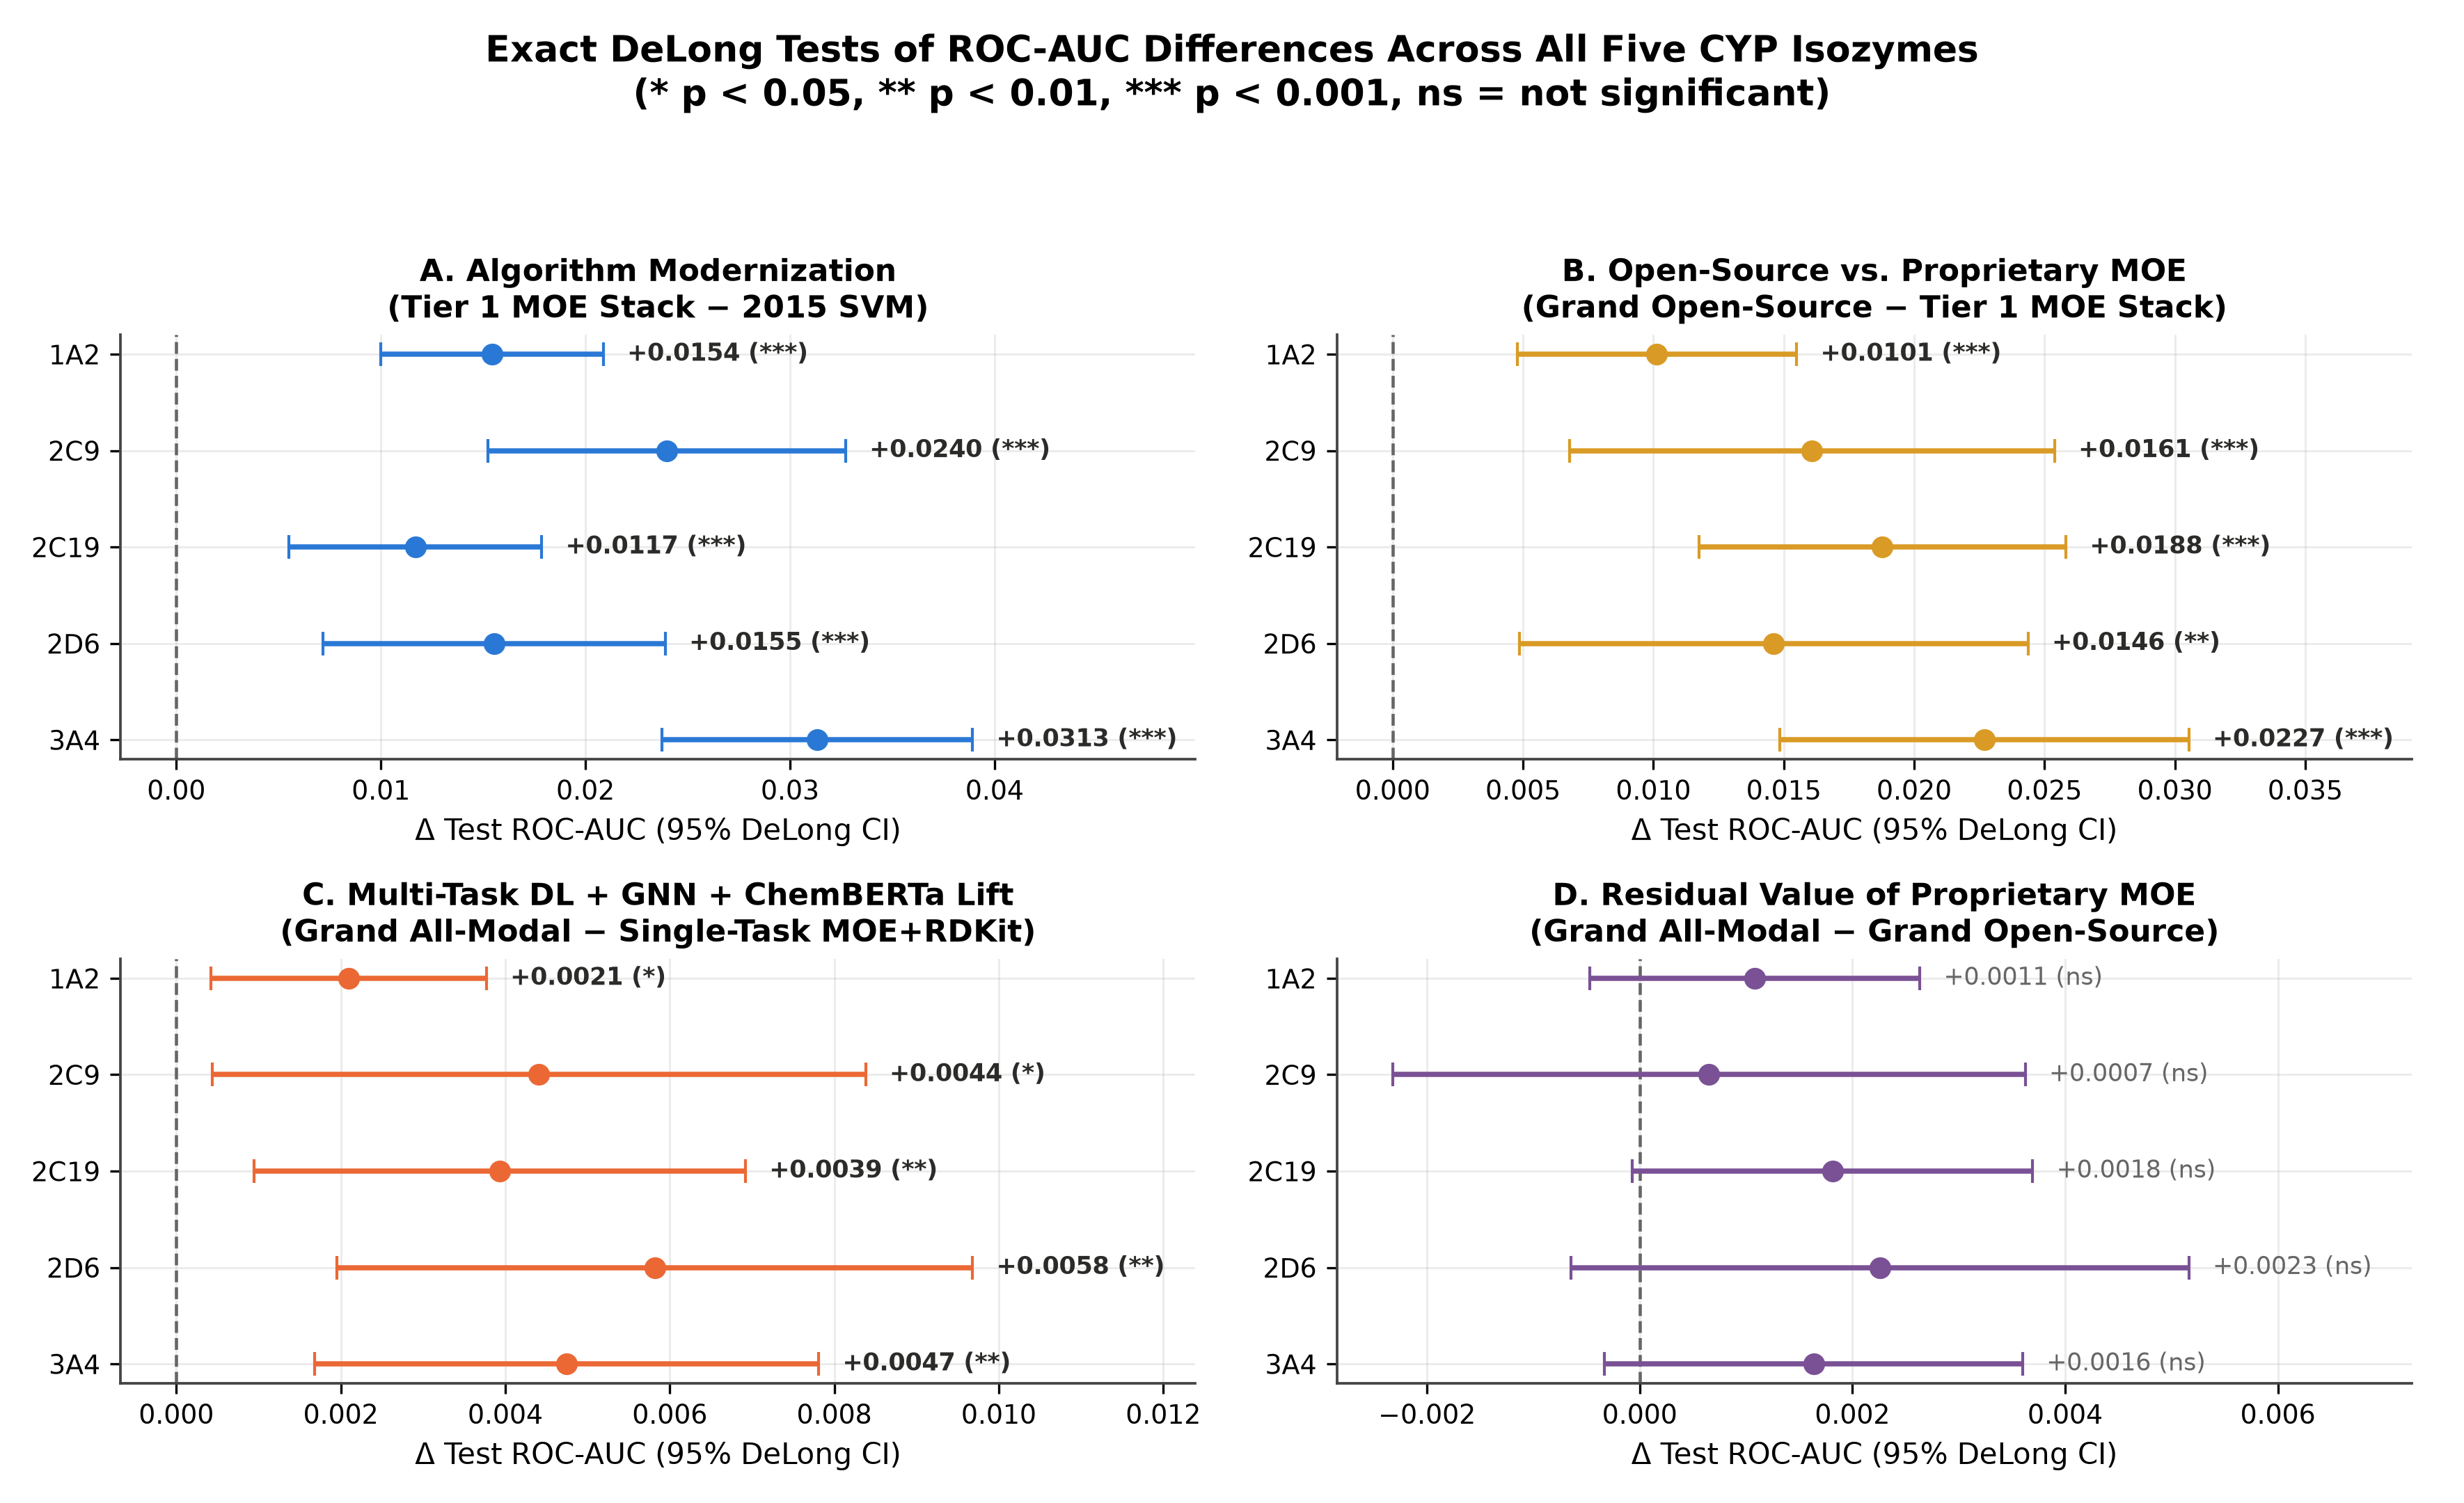
\includegraphics[width=0.95\textwidth]{img/fig4_delong_forest.png}
  \caption{Exact DeLong $\Delta$ROC-AUC forest plots (95\% CI) for four headline hypotheses across all five isozymes.}
  \label{fig:delong}
\end{figure}

\begin{figure}[htbp]
  \centering
  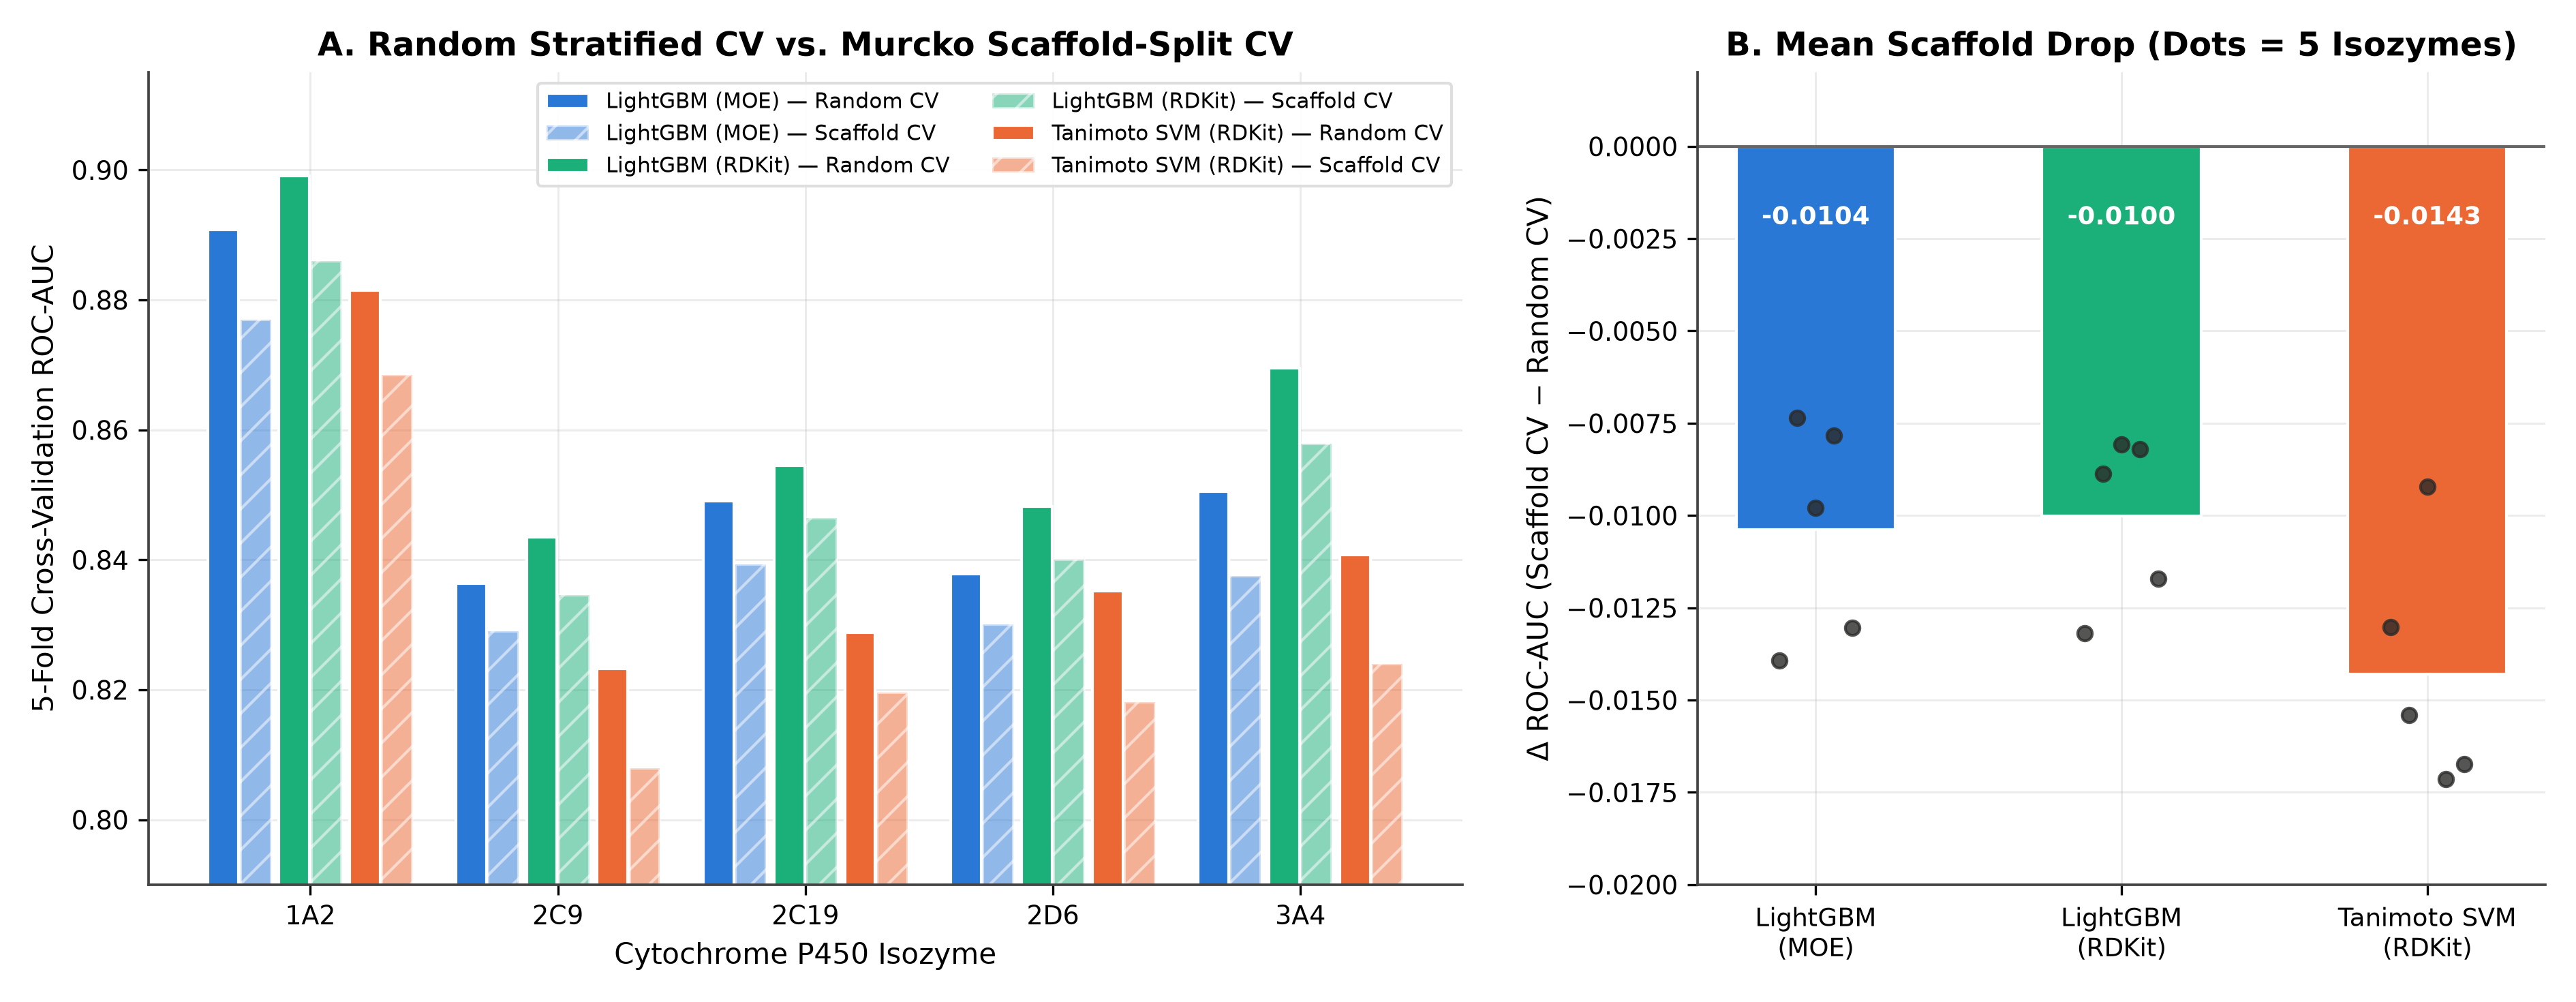
\includegraphics[width=0.95\textwidth]{img/fig5_scaffold_generalization.png}
  \caption{Random Stratified CV vs.\ Murcko Scaffold-Split CV across all five isozymes.}
  \label{fig:scaf}
\end{figure}

\begin{figure}[htbp]
  \centering
  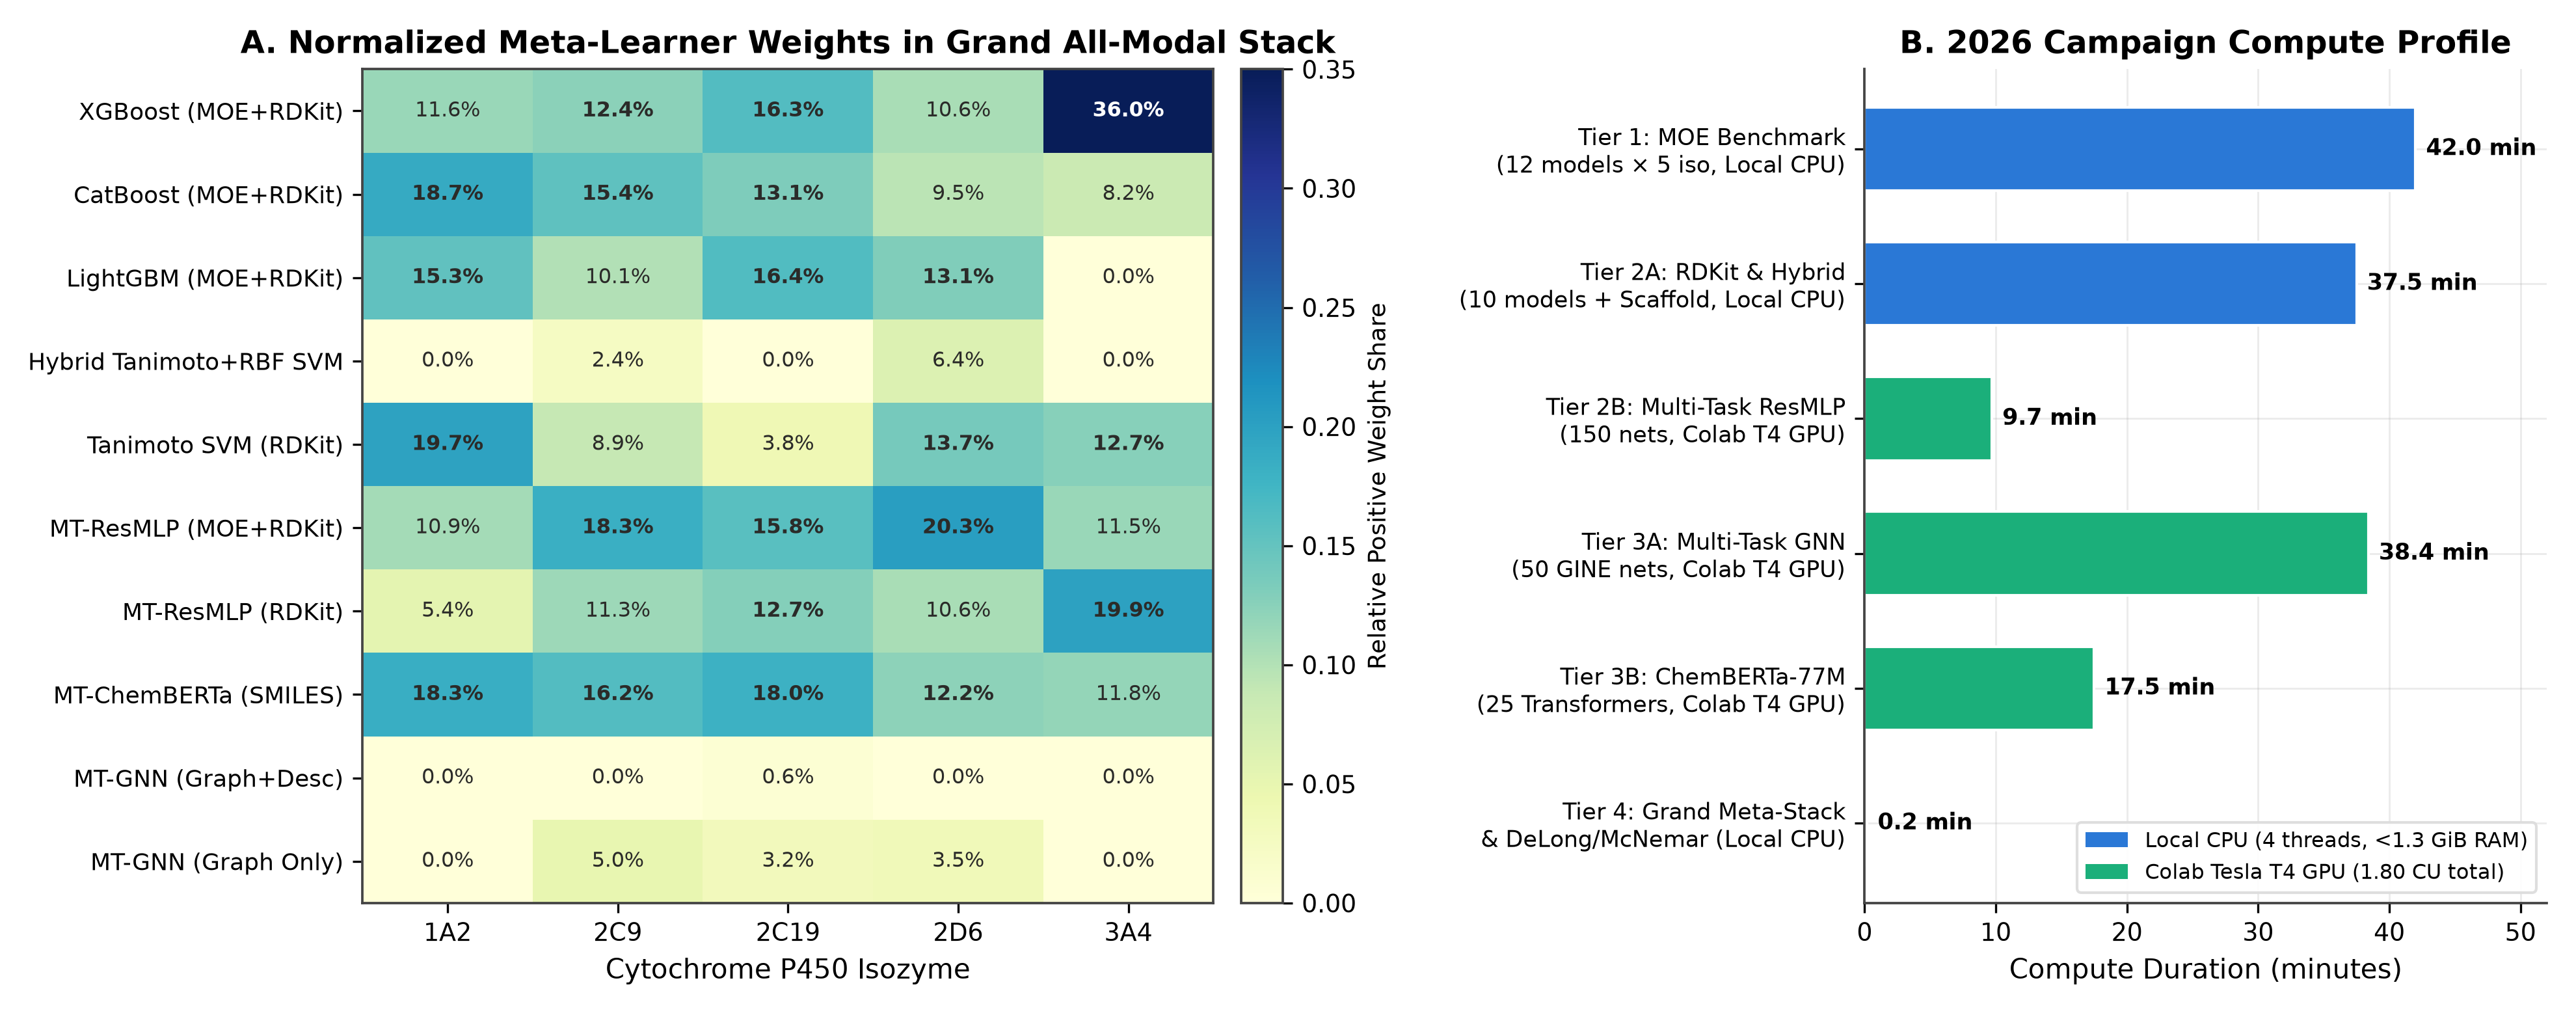
\includegraphics[width=\textwidth]{img/fig6_multimodal_weights_and_compute.png}
  \caption{(A) Normalized positive stacking weights in \texttt{Grand\_AllModal\_Stack}. (B) Compute duration across local CPU (4 threads, $<$1.3\,GiB RAM) and Colab Tesla T4 GPU (1.80 compute units total).}
  \label{fig:weights}
\end{figure}

\section{Discussion: Attributing Uplift and AI-Coordinated Throughput}
Decomposing the decade's +0.0375 ROC-AUC gain shows that modern tabular methods and open-source cheminformatics representations account for $\sim 89\%$ of the predictive uplift, while GPU-accelerated multi-task deep learning, GNNs, and pretrained molecular transformers contribute the final statistically significant $+11\%$ (+0.0042 AUC, with the strongest transfer on data-scarce CYP 2D6).

Equally striking is the shift in both hardware capacity and research throughput. In 2014--2015, the original notebooks ran on the \textbf{AWS EC2 Free Tier} (\texttt{t1.micro}/\texttt{t2.micro}: 1 vCPU, 613\,MiB--1\,GiB RAM, throttled to a 10\% baseline vCPU once burstable credits burned out after $\sim 30$ minutes), causing RBF-kernel SVM cross-validation sweeps across the five isozymes to run overnight or across multiple days. Moreover, the 2--3 semesters ($\sim 9$--12 months) invested in the 2015 thesis encompassed far more than model runtime: it meant simultaneously learning Python, Linux command-line tooling, AWS cloud administration, \LaTeX, MOE, cheminformatics, and graduate Pharmaceutical Sciences coursework. By contrast, in 2026—with domain judgment already in place—AI-coordinated hybrid execution across a 4-thread local mini PC and an on-demand Colab Tesla T4 GPU (1.80 compute units) compressed 30 model variants, $>1{,}000$ CV fits, automated zero-leakage auditing, OOM/dtype debugging, exact DeLong/McNemar testing, and seven 300-DPI figures into roughly \textbf{3.5 hours of wall-clock time} ($\sim 2.4$ compute-hours run largely in parallel). All new code, CSVs, prediction archives, and figures are stored cleanly outside the original thesis files, ready for standalone publication or future extension.

\end{document}
